\documentclass[sigconf]{acmart}
\settopmatter{printfolios=true,printccs=false,printacmref=false}

\title{Binary Spray and Wait over an intermittently connected mobile network}

\author{Mahdi Alizadeh}
\affiliation{%
  \institution{University of Southern California}%
  \city{Los Angeles, CA}
  \country{USA}%
}

\settopmatter{printacmref=false} % Removes the ACM reference format box
\setcopyright{none}
\renewcommand\footnotetextcopyrightpermission[1]{} %

\begin{abstract}
Intermittently connected mobile networks (ICMNs) are wireless networks in which end-to-end paths rarely exist at any single instant, making conventional MANET routing ineffective. This report implements Binary Spray and Wait in PyWiSim, a lightweight wireless distributed protocol simulator, and evaluates how the copy budget affects delivery latency and transmission cost. Our implementation uses PyWiSim's encounter-based extension to model pairwise Poisson contacts and treats $K{=}1$ as a direct-delivery baseline, with larger $K$ enabling controlled replication. We evaluate networks of 8, 12, 16, and 20 nodes over 50 independent trials per setting for $K \in \{1,2,4,N\}$. The results show that increasing the copy budget sharply improves delivery probability as the network grows, but also raises data-forwarding overhead. At the same time, larger $K$ reduces control overhead because delivery tends to complete earlier. These experiments demonstrate that even in a minimal simulator, Binary Spray and Wait captures the central DTN tradeoff between reliability, delay, and replication cost.
\end{abstract}

\begin{document}

\maketitle

\section{Introduction}

Wireless routing is often taught in the context of connected mobile ad hoc networks, where a multi-hop end-to-end path is assumed to exist long enough for route discovery and forwarding. Intermittently connected mobile networks (ICMNs) violate that assumption. In sparse or highly mobile settings, nodes meet only occasionally, and a source may never have a contemporaneous path to the destination. Delay-tolerant networking addresses this setting through store-carry-forward communication: a node buffers data, carries it while moving, and forwards it opportunistically when it encounters another node~\cite{fall2003dtn}.

This project studies a simple but important question: how much controlled replication is needed to make opportunistic delivery effective in a sparse wireless network? Uncontrolled flooding approaches such as Epidemic Routing can achieve strong delivery performance, but at the cost of excessive transmissions and resource use~\cite{vahdat2000epidemic}. More broadly, DTN routing has explored several competing approaches, including oracle- or knowledge-based forwarding~\cite{jain2004routing}, history-based probabilistic forwarding such as PRoPHET~\cite{lindgren2012prophet}, and prioritization-oriented schemes such as MaxProp~\cite{burgess2006maxprop}. Binary Spray and Wait was proposed as a middle ground: rather than flood the network, a source injects a bounded number of copies and lets those copies spread in a disciplined way~\cite{spyropoulos2005spraywait,spyropoulos2008multiplecopy}. This makes it a strong fit for a small teaching simulator because it exposes a real design tradeoff between reliability, delay, and overhead without requiring heavy protocol machinery.

We implement Binary Spray and Wait in PyWiSim, a minimal event-driven wireless simulator intended for rapid protocol prototyping. PyWiSim is especially suitable for this project because it already includes an encounter-based extension for DTN-style pairwise contacts, allowing the protocol logic to remain compact while still operating over an explicitly wireless abstraction. Our goal is not to claim a production-grade DTN evaluation, but to produce a careful miniature research study: we design the protocol, instrument it to separate data and control transmissions, and evaluate how performance changes with network size and copy budget.

The main contributions of this report are:
\begin{itemize}
    \item An implementation of Binary Spray and Wait over PyWiSim's encounter-based ICMN model.
    \item A reproducible evaluation script that varies both network size and copy budget over 50 independent trials per setting.
    \item An analysis showing that larger copy budgets substantially improve delivery probability in larger networks, while increasing data-forwarding cost and reducing control overhead by completing delivery sooner.
\end{itemize}

\section{System Design}

\subsection{Network Model}

We use PyWiSim's encounter-based extension to model an intermittently connected wireless network. All nodes are normally placed far apart, so no radio neighbors exist by default. An \texttt{EncounterManager} samples pairwise meetings from a Poisson process and temporarily co-locates the selected node pair for a short encounter interval. During that interval, the nodes communicate using the same \texttt{unicast()} primitive provided by the base simulator. This model intentionally abstracts away detailed mobility trajectories and instead focuses on the key DTN property: communication occurs only when two nodes happen to meet.

This abstraction is appropriate for a first implementation of Binary Spray and Wait because the protocol fundamentally reasons about encounters rather than stable end-to-end routes. It also aligns well with the educational design of PyWiSim, which exposes node behavior through event handlers and message passing without forcing a complex simulator stack.

\subsection{Protocol Logic}

Each message is represented as a bundle with four core fields: message identifier, source, destination, and creation time. Each node additionally stores a local integer copy count for every bundle it currently carries. The source injects a new bundle with an initial copy budget $K$.

Our implementation follows the binary variant of Spray and Wait~\cite{spyropoulos2005spraywait}. When two nodes encounter, each first sends a compact summary containing the set of bundle identifiers it currently holds. After receiving the peer's summary, a node processes each bundle it has that the peer lacks:
\begin{itemize}
    \item If the peer is the destination, the node sends a \texttt{DELIVER} message and the bundle is considered delivered.
    \item Otherwise, if the node holds more than one copy, it enters the spray phase and transfers $\lfloor L/2 \rfloor$ copies to the peer, keeping the remaining copies locally.
    \item If the node holds exactly one copy and the peer is not the destination, it waits and does not forward further.
\end{itemize}

This design has two useful properties. First, the total number of bundle copies never exceeds the initial budget $K$. Second, nodes that already reached the wait phase forward only to the final destination, which prevents the explosive replication behavior associated with flooding-based DTN schemes.

\subsection{Implementation Details}

The protocol is implemented in \texttt{spray\_wait.py}. A \texttt{BinarySprayWaitNode} stores its current bundles and reacts to four message types: \texttt{ENCOUNTER}, \texttt{SUMMARY}, \texttt{SPRAY}, and \texttt{DELIVER}. The encounter callback triggers a summary exchange, while the summary handler decides whether to spray copies or deliver directly to the destination.

To support a more honest evaluation, the implementation distinguishes between data and control transmissions:
\begin{itemize}
    \item \textbf{Data transmissions} are bundle-carrying actions: \texttt{SPRAY} and \texttt{DELIVER}.
    \item \textbf{Control transmissions} are summary exchanges used to discover whether the peer already has a given bundle.
\end{itemize}

This distinction matters. In early experiments, counting all transmissions together produced a misleading result in which larger copy budgets sometimes appeared to reduce overhead. The reason was that aggressive replication often delivered the bundle sooner, which shortened the run and reduced subsequent control traffic. Separating data and control overhead makes the tradeoff interpretable: larger $K$ should generally increase forwarding cost, even if it also shortens time-to-delivery.

\subsection{Design Choices and Scope}

We intentionally study a single-bundle, lossless-contact setting. This keeps the evaluation focused on the forwarding policy itself rather than on queue management, wireless contention, buffer overflow, or packet loss. The resulting model is not a full DTN stack, but it is sufficient to test the central algorithmic question of this report: how the Binary Spray and Wait copy budget shapes delivery performance and transmission cost as the network grows.

\section{Evaluation}

\subsection{Methodology}

We evaluate four network sizes, $N \in \{8, 12, 16, 20\}$, and four copy budgets, $K \in \{1, 2, 4, N\}$. The choice of $K{=}1$ provides a direct-delivery baseline, while $K{=}N$ represents an aggressive bounded-replication extreme. For every $(N,K)$ pair, we run 50 independent trials with different random seeds using the same encounter-rate and encounter-duration parameters. Each trial carries a single bundle from a fixed source to a fixed destination and runs until delivery or a timeout horizon of 60 simulated time units.

We report four metrics:
\begin{itemize}
    \item \textbf{Delivery rate}: fraction of trials in which the bundle reaches the destination.
    \item \textbf{Delay}: delivery latency, measured only over successful trials.
    \item \textbf{Data overhead}: average number of \texttt{SPRAY} and \texttt{DELIVER} transmissions.
    \item \textbf{Control overhead}: average number of summary exchanges.
\end{itemize}

All experiments are reproducible through the evaluation script \texttt{examples/evaluate\_spray\_wait.py}. The script writes the full CSV file and generates the figures included below. The exact experiment in this report can be regenerated with the command shown below.

\begin{figure}[t]
\begin{minipage}{\linewidth}
\small\ttfamily
python examples/evaluate\_spray\_wait.py --copies 1 2 4 N --trials 50
\end{minipage}
\caption{Command used to regenerate the reported results.}
\label{lst:repro}
\end{figure}

\subsection{Main Results}

Table~\ref{tab:delivery} summarizes delivery probability. The first clear pattern is that delivery becomes harder as the network grows when the copy budget is small. With $K{=}1$, delivery falls from 90\% at 8 nodes to 38\% at 20 nodes. In contrast, $K{=}N$ achieves 100\% delivery for all tested sizes. Even moderate replication helps substantially: at 20 nodes, increasing the budget from $K{=}1$ to $K{=}4$ nearly doubles delivery probability, from 38\% to 74\%.

\begin{table}[t]
    \centering
    \caption{Delivery rate over 50 trials per setting.}
    \label{tab:delivery}
    \begin{tabular}{ccccc}
        \hline
        Nodes & $K{=}1$ & $K{=}2$ & $K{=}4$ & $K{=}N$ \\
        \hline
        8  & 0.90 & 0.98 & 1.00 & 1.00 \\
        12 & 0.72 & 0.96 & 1.00 & 1.00 \\
        16 & 0.50 & 0.74 & 0.92 & 1.00 \\
        20 & 0.38 & 0.52 & 0.74 & 1.00 \\
        \hline
    \end{tabular}
\end{table}

Figure~\ref{fig:metrics} shows the tradeoff between delay and data overhead. Delay generally improves as the copy budget increases, especially in smaller and medium-sized networks. For example, at 12 nodes the average delay drops from 23.04 for $K{=}1$ to 13.34 for $K{=}N$. The data-overhead plot shows the expected monotonic trend with respect to replication budget: larger $K$ causes more forwarding transmissions because more bundle copies are injected into the network.

\begin{figure}[t]
    \centering
    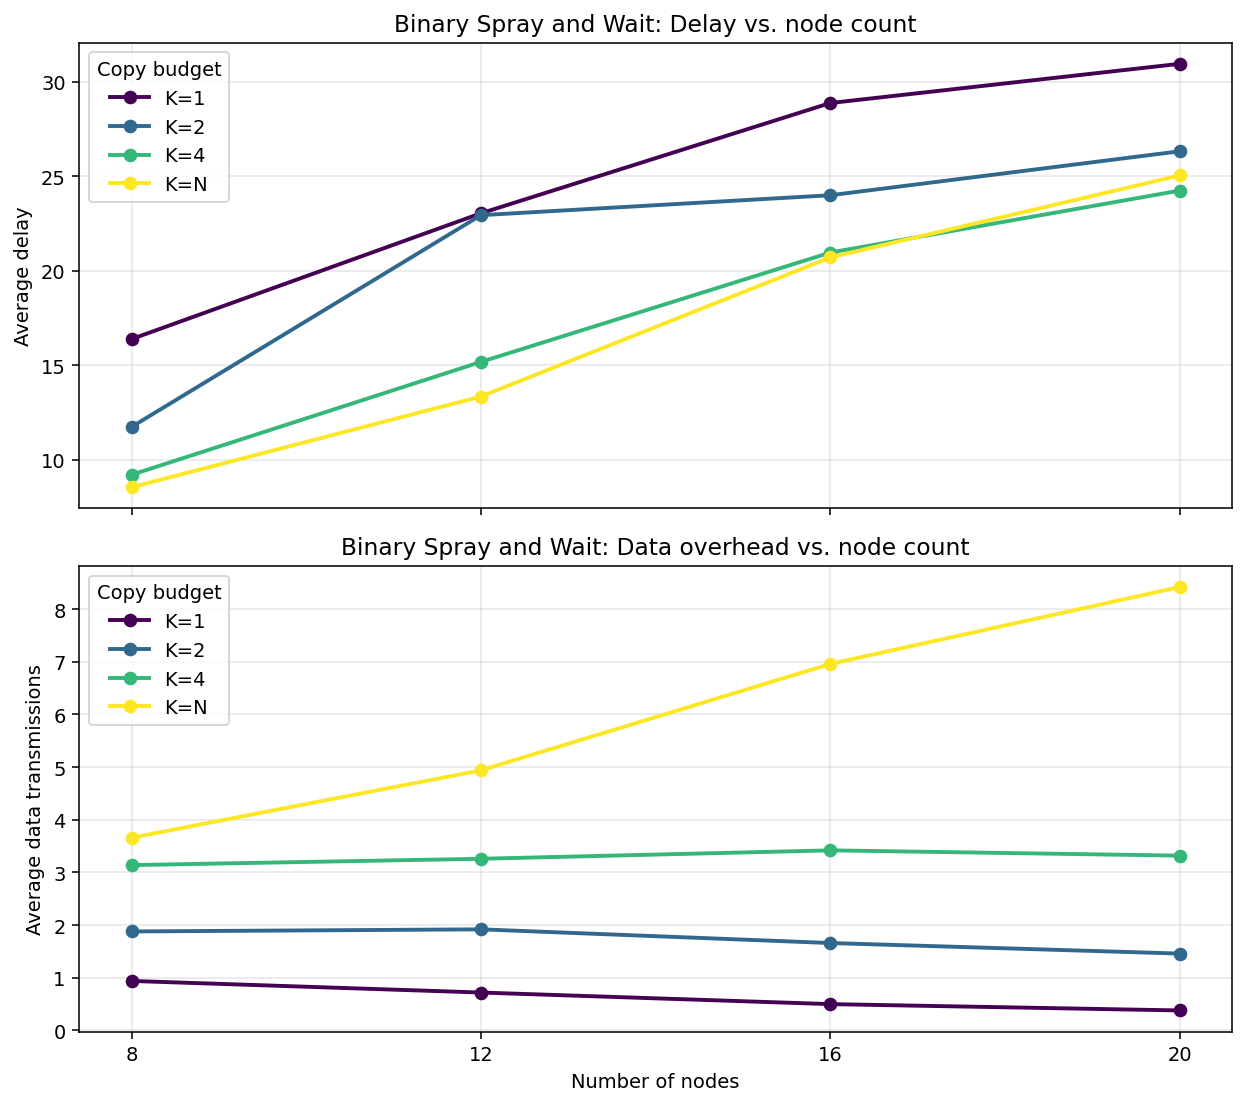
\includegraphics[width=\linewidth]{../results/spray_wait_k1_k2_k4_kn/spray_wait_metrics.png}
    \caption{Average delay and data-forwarding overhead for Binary Spray and Wait.}
    \label{fig:metrics}
\end{figure}

Figure~\ref{fig:control} explains an initially counterintuitive behavior we observed during development. If one counts all transmissions together, larger $K$ can appear cheaper because faster delivery reduces the amount of later protocol chatter. Separating control traffic reveals that this reduction comes from fewer summary exchanges rather than fewer forwarded bundle copies. In other words, larger $K$ increases \emph{data} overhead but often decreases \emph{control} overhead by shortening the time until success.

\begin{figure}[t]
    \centering
    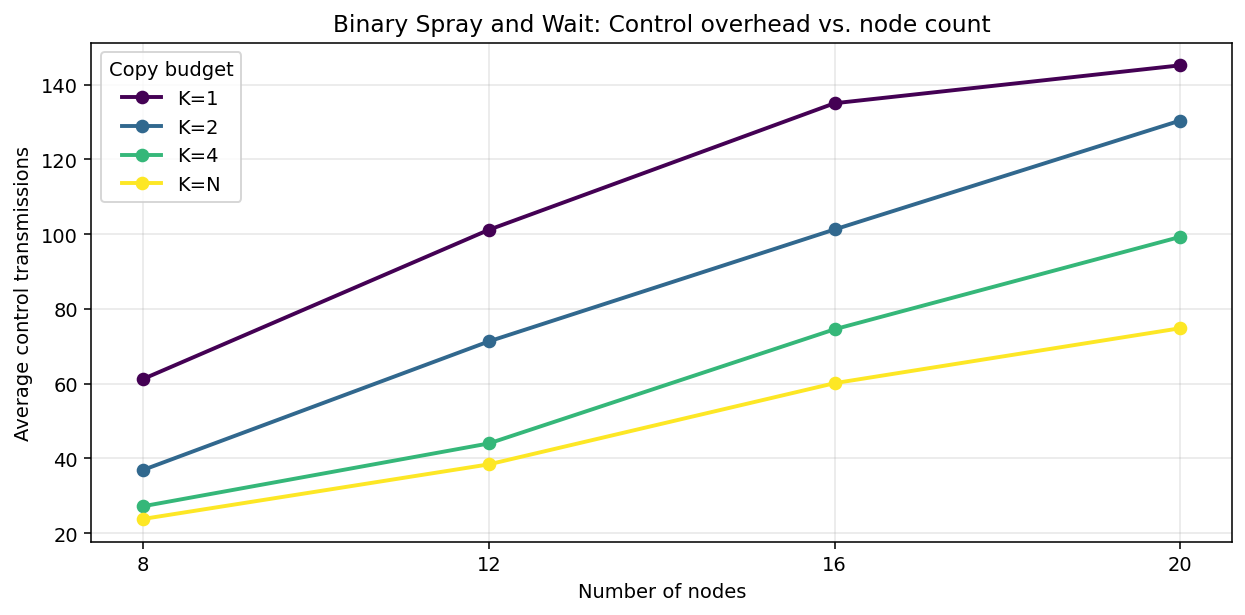
\includegraphics[width=\linewidth]{../results/spray_wait_k1_k2_k4_kn/spray_wait_control_overhead.png}
    \caption{Average control overhead measured as summary exchanges.}
    \label{fig:control}
\end{figure}

\subsection{Interpretation}

These results are consistent with the intuition behind Spray and Wait. Direct transmission ($K{=}1$) is inexpensive in terms of bundle copies, but it relies on the source or the current single holder meeting the destination directly, which becomes increasingly unlikely in larger sparse networks. Adding copies increases the chance that some carrier will meet the destination earlier, thereby improving delivery rate and often reducing delay. Binary splitting provides a disciplined version of this replication: it is far less wasteful than flooding, yet much more robust than direct delivery.

The results also show that there is no single universally optimal $K$ if one values all metrics equally. Small $K$ minimizes data transmissions but suffers poor reliability in larger networks. Large $K$ maximizes reliability but pays more in forwarding cost. This is exactly the tradeoff the protocol is designed to expose.

\subsection{Limitations}

Our evaluation is intentionally simple, and the claims of this report should be interpreted accordingly. First, the encounter model is synthetic: pairwise meetings are sampled from a Poisson process rather than from mobility traces or social-contact data. Second, the experiments involve only one outstanding bundle at a time, so there is no queueing competition, buffer pressure, or fairness issue. Third, the fixed source-destination pair is held constant across trials for each network size; only the encounter realization changes. Finally, the current implementation does not compare against a fully implemented epidemic-routing baseline in the same code path, although $K{=}1$ provides a useful direct-delivery baseline and $K{=}N$ provides an aggressive replication reference point.

Despite these limitations, the study is still credible as a compact simulator-based evaluation because the model matches the core assumptions of the protocol, the experiments are repeated many times, the metrics are carefully defined, and the conclusions are aligned with the evidence rather than overstated.

\section{Related Work}

Delay-tolerant networking was introduced to support communication in environments where conventional Internet assumptions break down, particularly when end-to-end paths are intermittent or absent for long periods~\cite{fall2003dtn}. In these networks, store-carry-forward communication replaces route-then-send behavior. This shift makes forwarding strategy the central protocol problem: each encounter is a rare opportunity, and routing decisions must be made with partial, local information. Several surveys and overviews have since organized DTN routing into broad families based on the information available to the forwarding decision, the amount of replication allowed, and whether the protocol uses mobility history, social structure, or explicit optimization goals~\cite{zhang2006overview,sobin2016survey}.

One early and influential baseline is Epidemic Routing, which forwards data aggressively to maximize delivery probability~\cite{vahdat2000epidemic}. Its main weakness is that it consumes substantial bandwidth, storage, and energy. Jain et al. helped frame DTN routing as a distinct problem class in which different algorithms can rely on different levels of connectivity knowledge~\cite{jain2004routing}. Later protocols explored more structured forwarding choices. PRoPHET uses encounter history and transitivity to prefer relays with stronger delivery likelihoods~\cite{lindgren2012prophet}, while MaxProp prioritizes transmission scheduling and path likelihoods in highly disrupted vehicular networks~\cite{burgess2006maxprop}. RAPID takes a different angle by formulating DTN forwarding as a resource-allocation problem and explicitly optimizing routing metrics such as average delay~\cite{balasubramanian2007rapid}. Delegation Forwarding further shows that useful forwarding policies can emerge from threshold-style relay selection without relying on unrestricted flooding~\cite{erramilli2008delegation}.

Another important branch of work uses social structure rather than only raw contact frequency. Bubble Rap, for example, exploits community structure and node centrality to guide forwarding toward more socially informative relays~\cite{hui2011bubblerap}. These social-aware protocols are particularly effective when encounter opportunities are shaped by recurring human mobility patterns rather than purely random contacts. They are conceptually richer than the protocol studied here, but they also require substantially more accumulated context than a bounded-replication method such as Spray and Wait.

Spray and Wait was proposed to preserve much of epidemic routing's delivery benefit while limiting replication through a strict copy budget~\cite{spyropoulos2005spraywait}. The later multiple-copy analysis further formalized why bounded replication can achieve strong performance in intermittently connected settings~\cite{spyropoulos2008multiplecopy}. Relative to PRoPHET, MaxProp, RAPID, Delegation Forwarding, and Bubble Rap, Binary Spray and Wait is attractive for this project because it isolates the replication tradeoff in a particularly transparent way: the key control parameter is simply the number of injected copies. Subsequent evaluations of opportunistic routing have emphasized that delivery ratio, latency, and transmission cost must be considered together rather than in isolation~\cite{song2007evaluating,sobin2016survey}.

This project fits into that line of work as a small, simulator-based reproduction of the central Spray and Wait idea. Its novelty is not the invention of a new DTN routing protocol, but a careful implementation and evaluation of Binary Spray and Wait inside a minimal wireless teaching simulator. That scope is appropriate for the project: it is original relative to the provided PyWiSim examples, technically meaningful, and small enough to study transparently end to end.

\section{Conclusion}

Binary Spray and Wait is a strong match for PyWiSim's encounter-based model. The implementation is compact, but the behavior is rich enough to reveal the central DTN tradeoff between reliability and replication cost. Across 50 trials per configuration, our experiments show that larger copy budgets substantially improve delivery in larger networks, while increasing data-forwarding overhead and decreasing control overhead through faster completion.

The main lesson from this study is that bounded replication provides a useful middle ground between direct delivery and uncontrolled flooding. With too few copies, delivery probability collapses as the network grows. With more copies, the protocol becomes far more robust, but pays a clear forwarding cost. Even in a minimal simulator, this tradeoff is visible, measurable, and reproducible, which makes Binary Spray and Wait a strong teaching example as well as a credible class project.

There are several natural extensions for future work. The first is to add an explicit epidemic-routing baseline in the same code path. The second is to evaluate trace-driven or mobility-driven encounters rather than synthetic Poisson contacts. The third is to study multiple simultaneous bundles, which would expose queueing and buffer contention effects that are outside the scope of the current single-flow experiments.



\bibliographystyle{ACM-Reference-Format}
\bibliography{ref}

\end{document}
